% This is a template for doing homework assignments in LaTeX

\documentclass{article} % This command is used to set the type of document you are working on such as an article, book, or presenation

\usepackage[margin=1in]{geometry} % This package allows the editing of the page layout
\usepackage{amsmath}  % This package allows the use of a large range of mathematical formula, commands, and symbols
\usepackage{graphicx}  % This package allows the importing of images
\usepackage{amsfonts}
\usepackage{enumitem}
\usepackage{listings}
\usepackage{hyperref}

% \setlength\parindent{0pt}

\newcommand{\question}[2][]{\begin{flushleft}
        \textbf{Question #1}: \textit{#2}

\end{flushleft}}
\newcommand{\sol}{\textbf{Solution}:} %Use if you want a boldface solution line
\newcommand{\maketitletwo}[2][]{\begin{center}
        \Large{\textbf{Project #1}
            
            ICCS315: Applied Algorithms} % Name of course here
        \vspace{5pt}
        
        \normalsize{Thanatad Anukoolprasert, Yuttasart Viratpan   % Your name here
        
        \today}        % Change to due date if preferred
        \vspace{15pt}
        
\end{center}}
\begin{document}
    \maketitletwo[]  % Optional argument is assignment number
    %Keep a blank space between maketitletwo and \question[1]
    
    \section*{Objective}
    The objective of this project is to benchmark two different type of data structures and compare different
    implementation of each type as well as their theoretical running time.
    The first type is resizable array where the following data structures are of interest
    \begin{itemize}
        \item Hashed Array Tree (Sitarski, 1996)
        \item Brodnik's resizable array non-superblock version (Brodnik et al., 1999)
        \item Brodnik's resizeable array superblock version (Brodnik et al., 1999)
    \end{itemize}
    The second type is hash table with 3 different collision resolution schemes, namely
    \begin{itemize}
        \item Chaining
        \item Open addressing
        \item Cuckoo hashing
    \end{itemize}
    
    For a lack of a better name, we are going to called both the data structures from \href{ https://sedgewick.io/wp-content/themes/sedgewick/papers/1999Optimal.pdf}{ Brodnik et al 1999}, Hashed Array Tree (HAT).
    More specifically, we are going to called Brodnik's HAT with non-superblock version \emph{Brodnik's HAT A} and the superblock version \emph{Brodnik's HAT B}.

    The dimensions of interest are the following
    \begin{itemize}
        \item Append latency
        \item Access latency
        \item Scan throughput
        \item Overall throughput
    \end{itemize}

    \section*{Method}
    We are going the implement the data structures above and benchmark them. Our implementation can be found here: \href{https://github.com/thanatadcs/apal-project}{ https://github.com/thanatadcs/apal-project}.
    We are going the measure running time in cycles using
    \emph{rdtsc} assembly instruction in x86 so that we are able to time quick operation like append with accurary.

    \subsection*{Remark on implementation}
    The implementation of \emph{get} function of Brodnik's HAT B is different from \emph{locate} function in the original paper.
    Namely, we cannot implement part of \emph{locate} function since there might be something wrong with the pseudocode in the paper,
    specifically \emph{$p=2^k - 1$} mentioned in the paper does not represent the number of data blocks before the $k$-th superblock as claimed,
    but it represent the number of elements before the $k$-th superblock instead. For this reason I have to implement my own way to get the number of
    data blocks before the $k$-th superblock. This can effect the running time of the \emph{get} function for Brodnik's HAT B. More information can be found in brodnik-hat-b.cpp.

    For Brodnik's HAT A and B, background-rebuilding optimization are also implemented so that we get $O(1)$ worst case append time. Brodnik's HAT B also utilized BSR assembly instruction in x86 to find
    the superblock number.

    \section*{Results and Discussion}
    \subsection*{Hashed Array Tree}
    All the number presented has the unit in cycles.
    \subsubsection*{Append latency}
    10 millions elements are appended and each append are timed, here are the statistics
    \begin{center}
        \begin{tabular}{|c|c|c|c|}\hline
            & Sitarski's HAT & Brodnik's HAT A & Brodnik's HAT B\\\hline
            mean &  59.7470848 & 48.3077336 & 46.6222048\\\hline
            standard deviation & 28458.271801239895  & 173.0441420332727 & 227.73642714240262\\\hline 
        \end{tabular}
    \end{center}
    For append latency, the ranking from best to worst running time is Brodnik's HAT B, Brodnik's HAT A, and Sitarski's HAT.
    This makes sense since Sitarski's HAT have to copy not only the pointer, but also all elements every time it's expand as compare to Brodnik's HAT A
    and B where only pointer need to be copy and since we do not need to copy the elements, background-rebuilding is possible which make this even better and in fact constant in term of append time.
    
    In another aspect, our results also follow the theoretical running time very well. For Sitarski's HAT, in theory append time is $O(1)$ amortized, so we can see that the mean
    is that not far off from Brodnik's A and B, but since this is amortized cost, the standard deviation can be very high since there might be spike in running time once in a while. Brodnik's A and B has $O(1)$ worst case append time so
    the standard deviation of both of these is very low. Here is a the plot for append time
    \begin{center}
        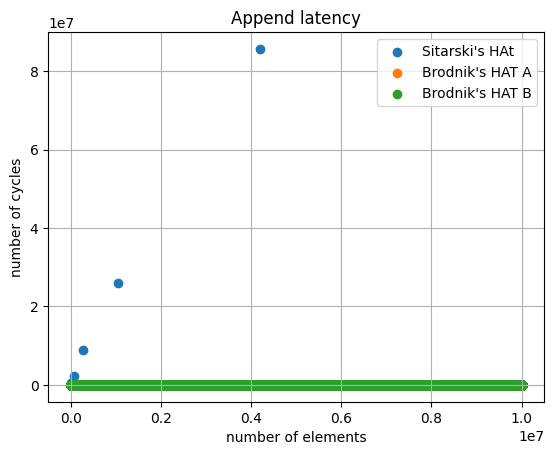
\includegraphics{graphics/hat_append.png}
    \end{center}
    which demostrated how the append time for Brodnik's A and B are constant.
    \subsubsection*{Access latency}
    10 millions elements are appended and all 10 millions elements get access through \emph{get} function.
    Each access is timed, here are the statistics
    \begin{center}
        \begin{tabular}{|c|c|c|c|}\hline
            & Sitarski's HAT & Brodnik's HAT A & Brodnik's HAT B\\\hline
            mean &  46.9125558 & 71.8199474 & 68.7515222\\\hline
            standard deviation & 31.649467204234057  & 35.97450913996233 & 90.24513109294548\\\hline 
        \end{tabular}
    \end{center}
    Here the ranking from best to worst are Sitarski's HAT , Brodnik's HAT B, and Brodnik's HAT A. Sitarski's HAT require little
    computation (a little bit of bitwise operation) to get to the index so it is the fastest. Brodnik's B is better than Brodnik's HAT A in
    their mean by a little bit which is a surprise since Brodnik's HAT B does not have any complex operation like square root. In term of standard deviation,
    Brodnik's HAT A clearly out perform Brodnik's HAT B since the running time is more consistant.

    In theory, Sitarski's HAT has $O(1)$ access time so it is not a surprise that it is very fast with low standard deviation.
    Brodnik's HAT B supposed far to be better than Brodnik's HAT A, since Brodnik's HAT B promise $O(1)$ access time where
    Brodnik's HAT A does not since it has to compute square root, but our results does not goes that way since Brodnik's HAT B and A
    relatively has similar running time in term of mean, but for Brodnik's HAT A clearly has a more consistant result.
    Here is the graph for access time
    \begin{center}
        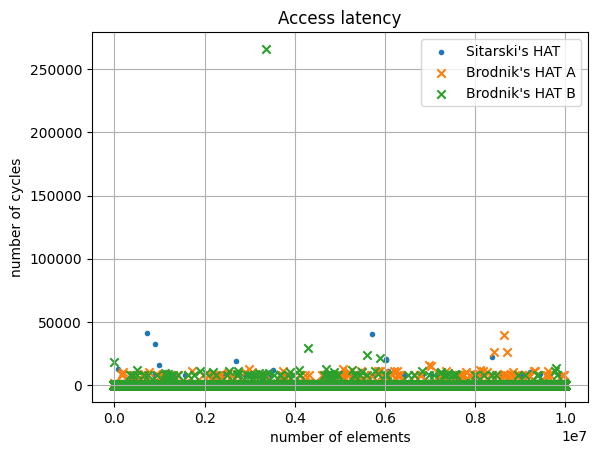
\includegraphics{graphics/hat_access.png}
    \end{center}
    which show how the access time for all 3 HATs looks relatively constant (except that Brodnik's HAT A access is not constant in theory, but is low enough to look like so).

    \subsubsection*{Scan throughput}
    1000 elements are appended and all the 1000 elements are accessed. The total time used to access all elements is measured and we do this for 1000 times.
    Here are the statistics. 
    \begin{center}
        \begin{tabular}{|c|c|c|c|}\hline
            & Sitarski's HAT & Brodnik's HAT A & Brodnik's HAT B\\\hline
            mean &  16439.928 & 38772.878 & 53974.224\\\hline
            standard deviation & 1509.39901776038  & 3611.297266234946 & 2422.0789396351224\\\hline 
        \end{tabular}
    \end{center}
    For scan throughput, ranking from best to worst is Sitarski's HAT, Brodnik's A, and Brodnik's B.
    Again similar to our access time, Sitarski's HAT perform the best. Brodnik's HAT A beat Brodnik's HAT B this time which is a
    surprise. Even though the access time for Brodnik's HAT A is not constant, but it is still relatively very low
    so it might also occur that Brodnik's HAT B access time get out performed by Brodnik's HAT A because of overhead.

    In term of theory, Sitarski follows the theoretical running time very well with constant low access time (because of simple bitwise).
    But for Brodnik's HAT A, even though in theory, we would say that it is worse than Brodnik's HAT B, but our results has shown that it can be better.

    Of course, it might also means that our Brodnik's HAT B is not optimized enough and we may have to do additional book keeping to make this more optimized.
    Another factor can also stem from the fact that our implementation is a bit different from that of the paper, in this case we might as well trying to find a better
    a better and faster way to compute the number of data blocks before a given superblock.

    \subsubsection*{Overall throughput}
    1000 elements are appended. The total time used to append all 1000 elements is measured and we do this for 1000 times.
    Here are the statistics
    \begin{center}
        \begin{tabular}{|c|c|c|c|}\hline
            & Sitarski's HAT & Brodnik's HAT A & Brodnik's HAT B\\\hline
            mean &  31624.766 & 26366.932 & 28797.736\\\hline
            standard deviation & 1774.3194777840883  & 1691.4454491280528 & 2090.277559154286\\\hline 
        \end{tabular}
    \end{center}
    For overall throughput, ranking from best to worst is Brodnik's HAT A, Brodnik's HAT B, and Sitarski's HAT.
    All three HATs does not have that far off running time in terms of mean and they have relatively the same standard deviation.

    This is according to the theory since all of the have $O(1)$ append time (Sitarski's is amortized), the overall throughput
    average out some bad running time for Sitarski's HAT, but still it cannot beat Brodnik's HAT A and B since both of these are constant worst case append time.
    
    \subsection*{Hash table}

    \section*{Conclusion}
    We have implemented and benchmark 3 versions of HATs and 3 versions of hash table.
    
    For HATs, we have found that Brodnik's HAT A and B does very well for append/overall throughput when compare to Sitarski's HAT this is partly due to
    the background-rebuilding optimization that has been implement for both of the former and the fact that the former does not copy over all the elements
    when expanding. For access/scan throughput, Sitarski's outperformed Brodnik's HAT A and B, this is because the former does only simple bitwise operation to figure out the index,
    but Brodnik's HAT A is more complex which involves square root which does not run in constant time and Brodnik's HAT B even though use some bitwise operation and BSR x86 assembly directly, but
    the arithmetics required can be heavy enough to weight it down, additional book keeping might be needed to make this better. Also noted that the modification from
    the original paper for the function used to access might also affect the running time.

    Also note that Brodnik's HAT A performed better than Brodnik's HAT B for scan throughput, even though Brodnik's HAT B promise better theoretical constant running time, but in this
    case our implementation might introduce some overhead to make this worse than the Brodnik's HAT A which does not have constant access, but access time can be low enough to beat the overhead for
    Brodnik's HAT B. This does show that even though the theory says that Brodnik's HAT B is better than Brodnik's HAT A, but our result show that this is not the case in practice.
    If we are taking in to account the ease of implementation for Brodnik's HAT A and our results for its performence, Brodnik's HAT A is better than Brodnik's HAT B in this case.

\end{document}
